\section{Evaluation}
\label{sec:eval}

% 5. Methodology and evaluation: how do you plan to evaluate whether your ideas
% work or your hypotheses are correct?

In my proposal I make three specific claims we must evaluate,
\textbf{To develop an intelligent (1) end-to-end deep learning compiler that can
automatically adapt (2) high-level programs to run on new hardware devices automatically
with (3) human level performance.}

We evaluated Relay on several systems (x86 CPUs, ARM CPUs, NVIDIA GPUs, Xilinx FPGAs) and over
  diverse vision and NLP workloads to demonstrate that (1) Relay enables \emph{composability} of
  graph-level optimizations, (2) Relay delivers \emph{performance} on inference tasks competitive
  with state-of-the-art frameworks (TensorFlow, PyTorch, MxNet), and (3) Relay provides
  \emph{portability} over difficult-to-compile-to hardware backends such as FPGAs

\subsection{Relay: A high-level IR for Deep Learning}
  In particular, our evaluation is composed of three parts:
  \begin{enumerate}
    \item \textbf{Relay enables composable optimizations}: Relay
      supports composing program transformations into multiple optimization tiers.
    \item \textbf{Relay provides competitive performance}: Despite increasing
      expressiveness, Relay's performance is competitive with the
      state of the art on popular models.
    \item \textbf{Relay handles challenging backends}: Relay can compile
      models to execute efficiently on a variety of
      backends, such as FPGA accelerators, which require quantization, layout
      optimizations, and bit-packing transformations.
    % \item \textbf{Relay supports expressive models}: It can compile models with complex control flow
    % like Char-RNN to a single lean binary, beating PyTorch inference performance by up to 3x.
  \end{enumerate}

  We evaluated the following vision models:
    \textit{Deep Q-Network (DQN)}, a DNN that achieved state-of-the-art performance
    on 49 Atari games in 2015;
    \textit{MobileNet}, a DNN designed for image recognition on mobile and
    embedded devices;
    \textit{ResNet-18}, a DNN for image recognition that achieved state-of-the-art
    performance on ImageNet detection tasks in 2015;
    \textit{VGG-16} (named for the Visual Geometry Group
    at Oxford), a CNN used for image recognition tasks
    \citep{dqn, mobilenet, resnet, vgg}.

  We evaluated the following NLP models:
    \textit{CharRNN}, a generator character-level
    RNN from a PyTorch tutorial;
    \textit{TreeLSTM}, a generalization of LSTMs to
    tree-structured network topologies;
    \textit{RNN, GRU, and LSTM}, a selection of models from the Gluon
    model zoo
    \citep{pytorch_rnn_tut, tree_lstm, gluon_model_zoo}.

  \subsection{Experimental Methodology}
  % Because we only evaluate inference in this paper,
  %   we frequently make use of random inputs to models when measuring
  %   performance.
  % There were two exceptions where we evaluated on real data because
  %   it was readily available: CharRNN and TreeLSTM.

  % % For models where the input is random,
  % %   we run 1000 timed iterations.
  % % Before the timed runs,
  % %   we run 8 untimed ``warm-up'' iterations to ensure any caching and JIT compilation
  % %   employed in lower levels of the stack are included in the 1000 timed runs.
  % % This way,st
  % %   the timed runs reflect the \textit{stable} performance of the system.
  % % For our purposes, ``performance'' refers to end-to-end framework time on
  % %   inference tasks (i.e., the time it takes to run a trained model) in a
  % %   single-machine setting.

  Our vision experiments from Chapter~\ref{ch:related} and Section~\ref{sec:perf-gpu} were run on a machine with an AMD Ryzen
    Threadripper 1950X 16-Core CPU,
    an NVidia 1080 Ti GPU,
    and 64 GB of RAM.
  Our NLP experiments from Section~\ref{sec:perf-gpu} were run on a machine with an AMD Ryzen
    Threadripper 1950X 16-Core CPU,
    an NVidia Titan-V GPU,
    and 64 GB of RAM.
  Our low-power vision experiments from Section~\ref{sec:low-power} were run on multiple edge-class ARM development boards: a RaspberryPi 3, a Firefly RK3399, and an Ultra-96 FPGA platform.
  We evaluated Relay's handling of accelerators on a VTA design with a
    $16\times16$ matrix-vector 8-bit tensor core clocked at 333MHz on the Ultra-96 platform.

  % In terms of software, we used
  %   Cuda version 10.0,
  %   CuDNN version 7.5.0,
  %   TVM commit \texttt{cefe07e2a}\footnote{NLP experiments required custom modifications that may be made public later},
  %   MxNet version 1.4.0,
  %   Pytorch version 1.0.1post2,
  %   and TensorFlow version 1.13.1.

  The Relay vision experiments utilized aggressively tuned TVM schedules on the GTX 1080 Ti GPU,
    improving performance significantly.
  % \subsection{Relay Enables Composable Optimizations}
  % \label{sec:optimizations}

  % \begin{figure}[h]
  %   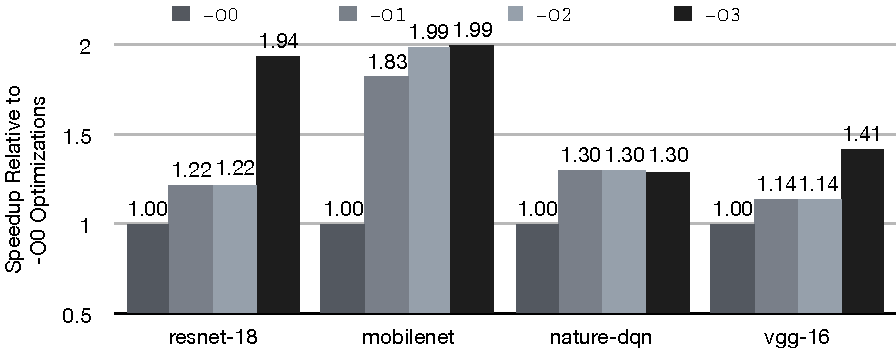
\includegraphics[width=0.5
  %   \textwidth]{fig/eval/optimization_levels.pdf}
  %   \caption{Speedup from increasing the number of graph transformations in Relay (\texttt{-O1}, \texttt{2}, \texttt{3}), relative to no optimizations at all (\texttt{-O0}). We show that, by composing passes, we can monotonically improve performance on vision benchmarks running on the NVIDIA GTX 1080 Ti.}
  %   \label{fig:opt-eval}
  % \end{figure}

  % We demonstrate that Relay can facilitate composable optimizations,
  % by evaluating vision workloads under incremental optimization levels, denoted \texttt{-On}:
  % \begin{itemize}
  %   \item \texttt{-O0} does not apply any program transformation passes.
  % % (it applies a single pass to translate the ``batch norm'' operator into simpler arithmetic
  % % operators but Relay{} has no other implementation of ``batch norm'').
  %   \item \texttt{-O1} applies an operator fusion pass.
  %   \item \texttt{-O2} additionally applies constant folding, using Relay{}'s interpreter to evaluate away operations on constants.
  %   \item \texttt{-O3} additionally applies four more passes:
  %       (1) \texttt{FoldScaleAxis}, which folds scaling operations into the axis options of other operators,
  %       (2) \texttt{AlterOpLayout}, which alternates operator layouts for better cache performance,
  %       (3) \texttt{CanonicalizeOps}, which canonicalizes the ``bias add'' operator in terms of expanding dimensions and broadcasting for further analysis,
  %       (4) \texttt{CommonSubexpElim}, which lifts common subexpressions.
  % \end{itemize}

  % Figure~\ref{fig:opt-eval} shows mean inference speedup relative to
  %   \texttt{-O0} as Relay applies optimizations more aggressively.
  % Average performance improves by up to 2$\times$ when all optimizations are applied.
  % Most networks benefit greatly from operator fusion.
  % Nature-DQN~\citep{dqn} has simple operators, which don't benefit from optimizations
  %   such as layout transform, explaining why its performance doesn't improve beyond \texttt{-O1}.
  % ResNet-18~\citep{resnet} and VGG-16~\citep{vgg} are two dense convolutional neural
  %   networks which benefit from \texttt{-03} optimizations.
  % These networks contain dense \texttt{conv2d} operators that benefit
  %   from the \texttt{AlterOpLayout} pass.
  % Overall, these results show that Relay lets us compose optimizations
  %   in a way that is beneficial to diverse workloads.

  \subsection{Relay Provides Competitive Performance}
  \label{sec:perf-gpu}

  \begin{figure}[h]
    % 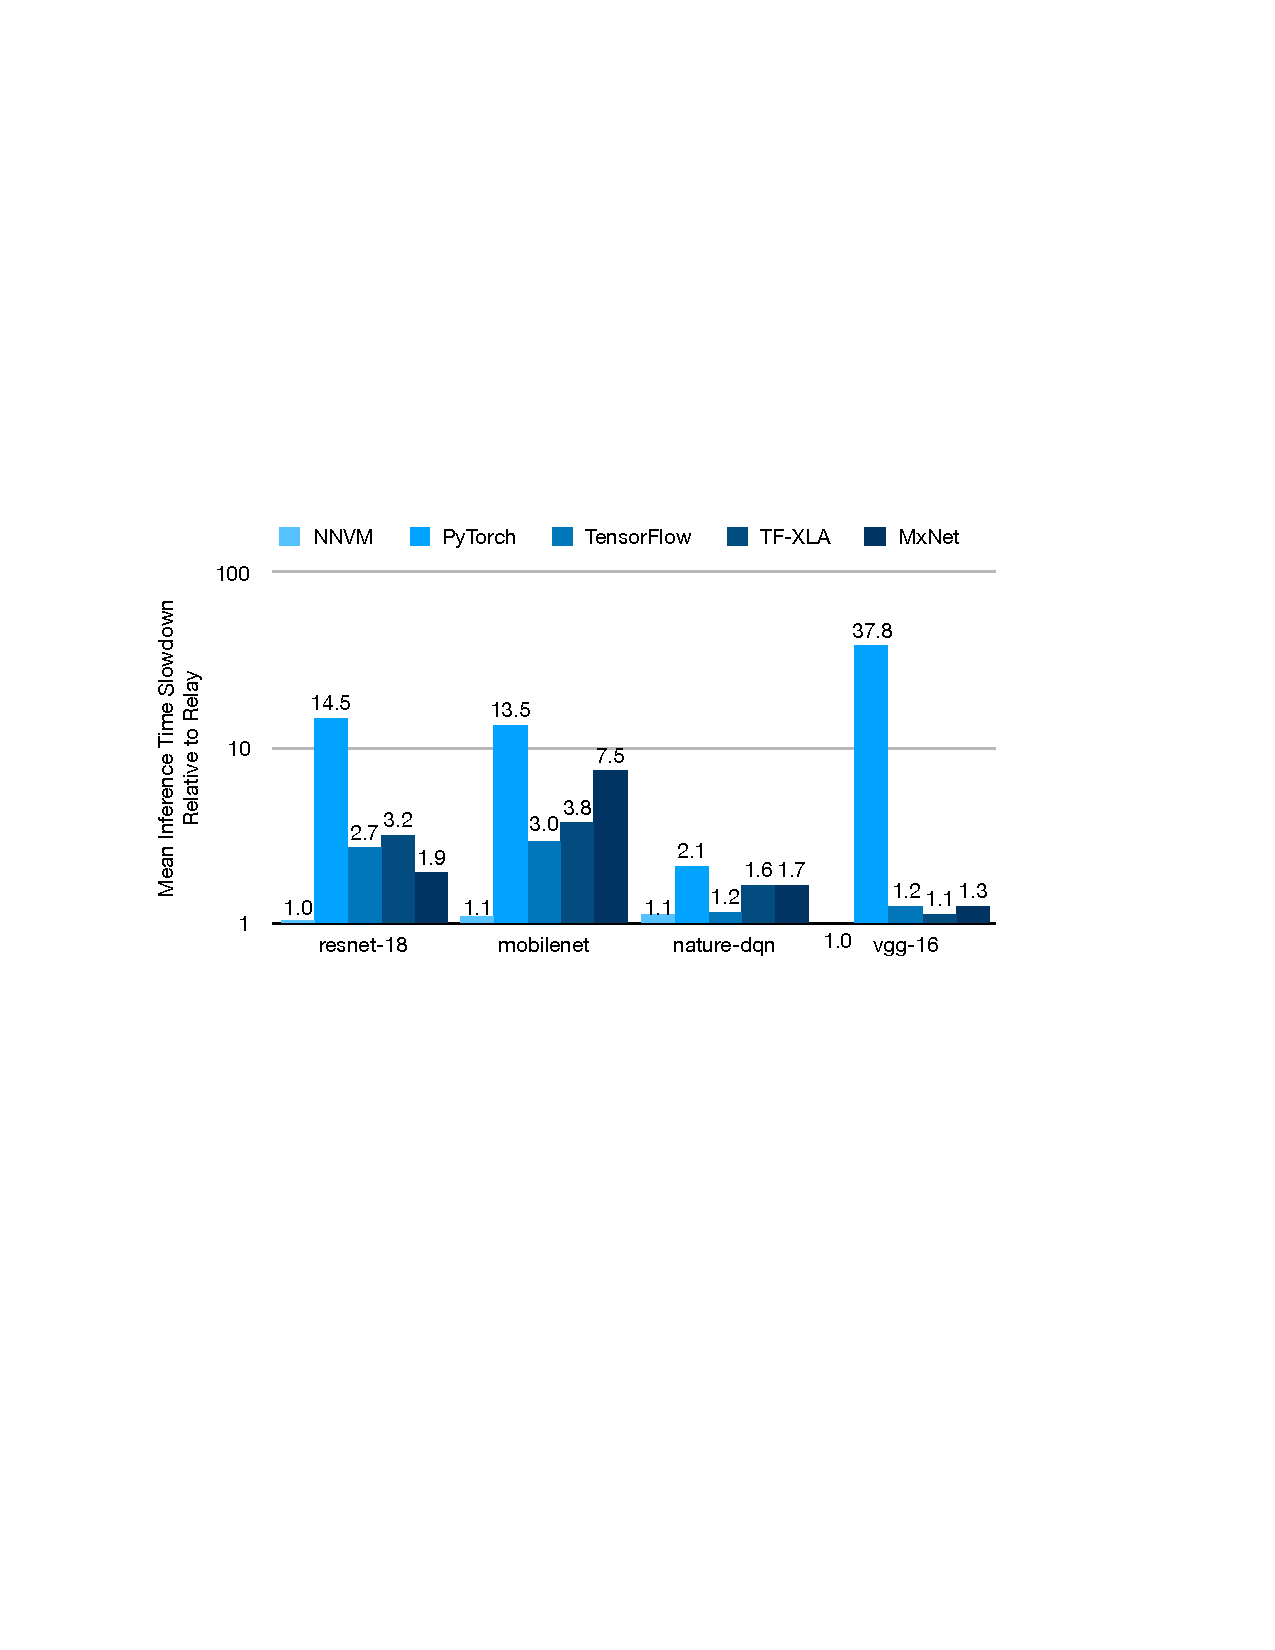
\includegraphics[width=0.6
    % \textwidth]{fig/eval/vision_1080Ti_relay.pdf}
    % \captionof{figure}{
    %   Inference slowdown of popular frameworks relative to Relay on vision
    %     benchmarks running on NVIDIA GTX 1080 Ti GPUs.
    %   Relay provides performance competitive to the state of the art.
    %   We ran 1000 trials for each model and used the AoT compiler.
    % }
    % \label{fig:vision-eval}
  \end{figure}

  \begin{figure}[h]
    % 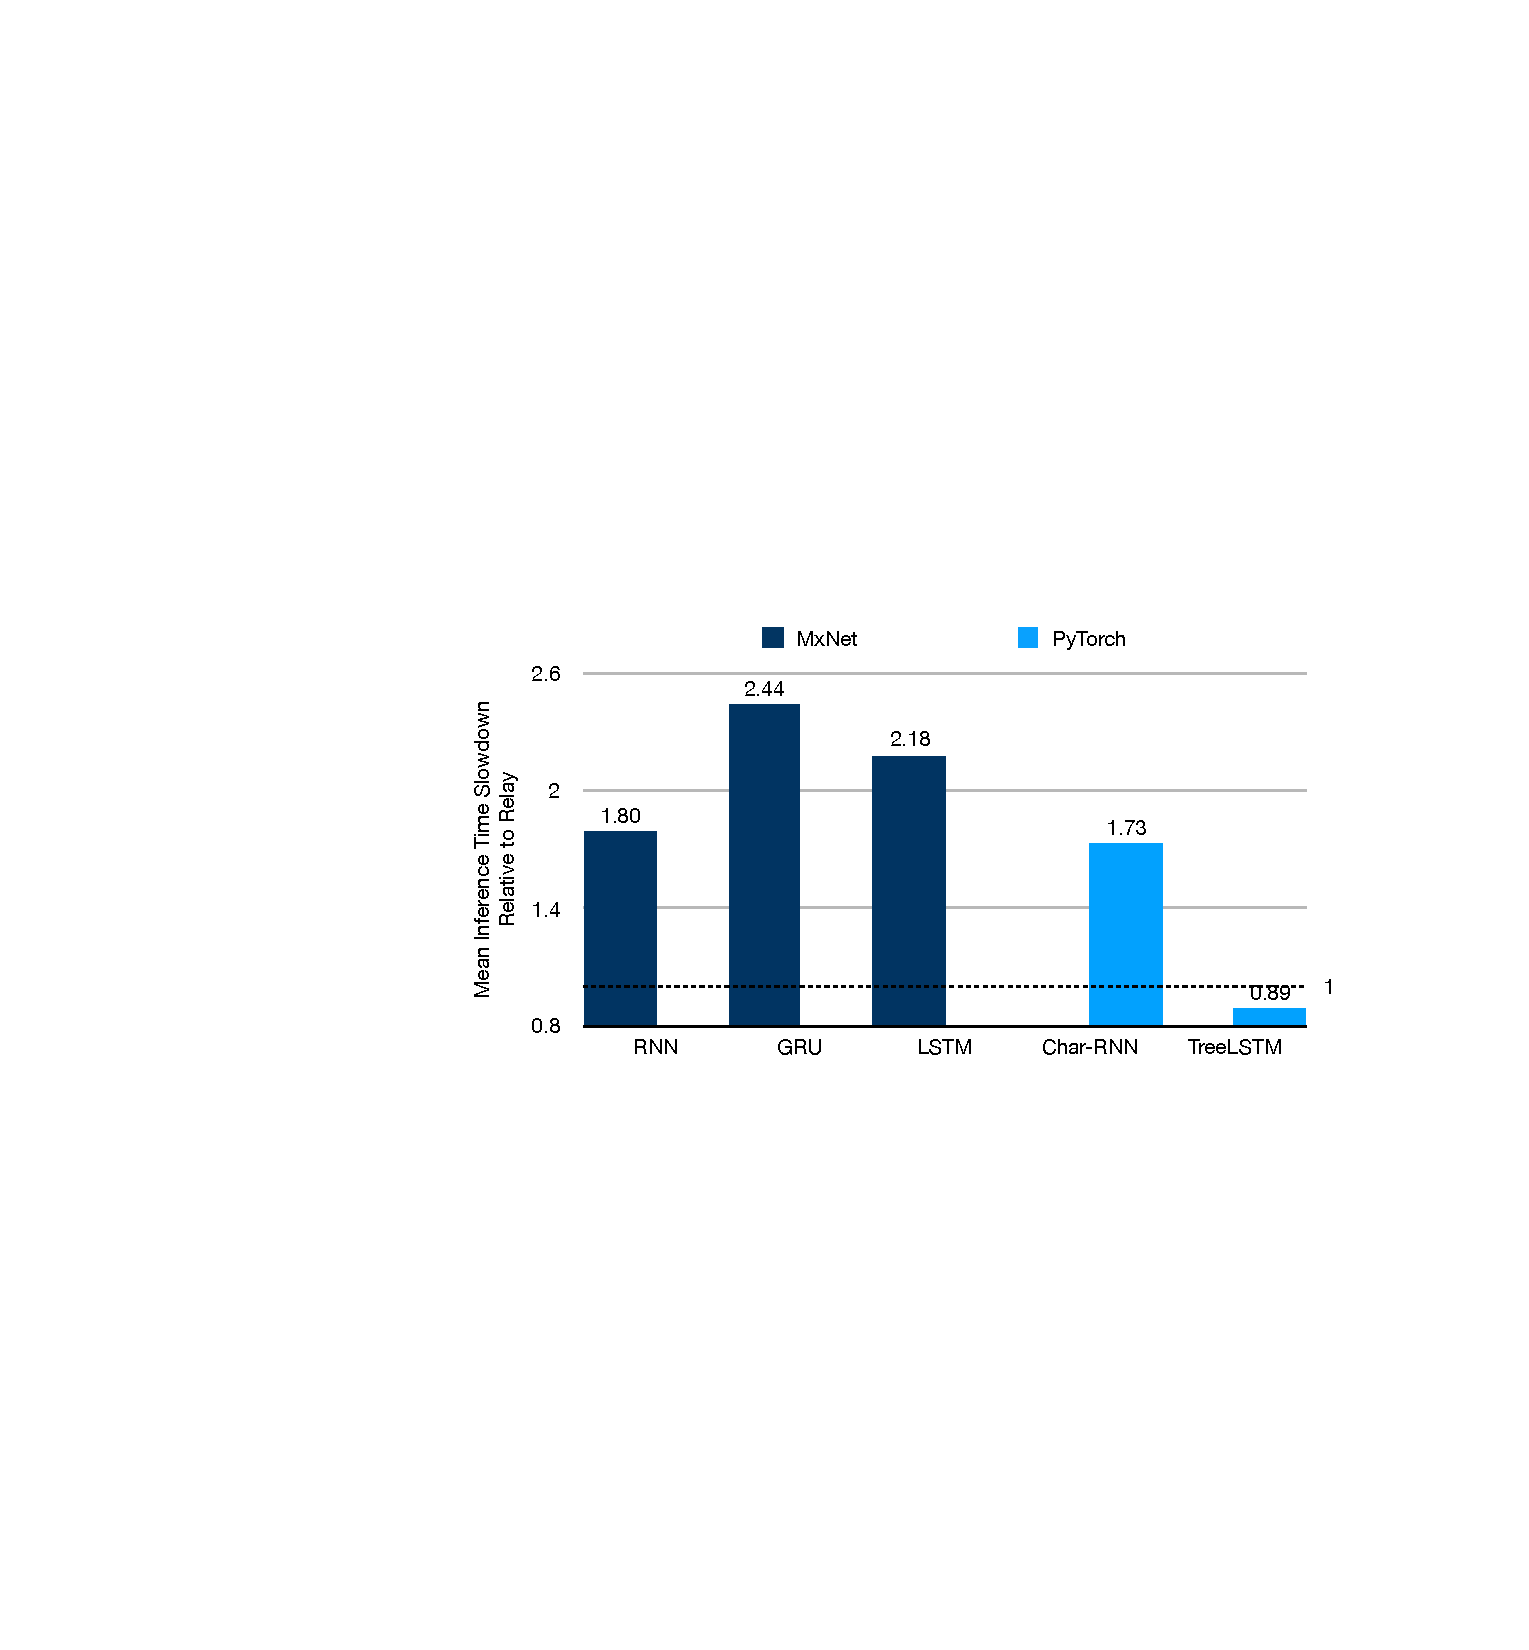
\includegraphics[width=0.6
    % \textwidth]{fig/eval/nlp_TitanV_relay.pdf}
    % \captionof{figure}{
    %   Inference slowdown relative to Relay on NLP benchmarks running on NVIDIA
    %     Titan-V GPUs.
    %   NLP workloads feature control flow,
    %     which makes them more challenging to optimize.
    %   Relay provides performance competitive to state of the art (up to
    %     2.4$\times$ speedup over MxNet on GRU).
    %   We ran 1000 trials for each model, except for CharRNN, on which we used 100 trials.
    % }
    % \label{fig:nlp-eval}
  \end{figure}

  An age-old story in compilers literature is that increasing expressivity
    impacts the global performance of the system.
  We set out to build zero-cost abstractions for Relay,
    governed by Stroustrup's principle, ``What you don't use, you don't pay
    for'' \citep{bjarne}.
  We demonstrate that we can achieve competitive performance on both CPUs and
    GPUs on a wide set of CNNs that are well supported by existing frameworks.
  We evaluated inference time for two classes of workloads: computer vision and natural language processing.
  We compared Relay (using our AoT compiler) to \nnvm,
    TensorFlow, TensorFlow-XLA (Accelerated Linear Algebra), PyTorch, and MxNet.
  We ran the vision and NLP workloads on GTX 1080 Ti and Titan-V GPUs, respectively.

  \paragraph{Vision Evaluation}
  Figure~\ref{fig:vision-eval} compares Relay against state of the art frameworks
    running vision workloads on a GTX 1080 Ti GPU.
  We ran each model with
    batch size 1, a common setting in inference tasks.
  Relay achieves performance on par with \nnvm,
    an existing deep learning graph compiler in use at Amazon.
  Relay outperforms TensorFlow, TensorFlow-XLA, MxNet and
    PyTorch on every benchmark.
  Relay's ability to do aggressive optimizations like operator
    fusion on long chains of operations, generating hardware
    specific implementations, enables it to outperform
    existing frameworks that don't perform inter-operator optimizations.

  \paragraph{NLP Evaluation}
  Figure~\ref{fig:vision-eval} compares Relay against state-of-the-art NLP models on a Titan-V GPU.
  Implementations of the NLP models were not available in all frameworks;
    we used MxNet baselines for RNN, GRU, and LSTM and PyTorch for Char-RNN and TreeLSTM.
  % We ran the models for 1000 iterations per input, except char-RNN, which we ran for 100 ???.
  % To run the RNN, GRU, and LSTM benchmarks in MxNet, and Char-RNN, and TreeLSTM
  %   in PyTorch.
  Relay performs better than MxNet on recursive models
    due to the fact they are implemented in Python using
    MxNet's looping constructs.
  PyTorch instead uses handwritten and heavily optimized
    C implementations of the recursive network cells.
  Due to this we perform slightly \emph{worse} than PyTorch.
  It is interesting to note that our pure Relay
    implementation performs competitively against
    the hand-optimized version.

  \subsection{Relay Handles Challenging Backends}
  \label{sec:low-power}

  \begin{figure}[h]
    % 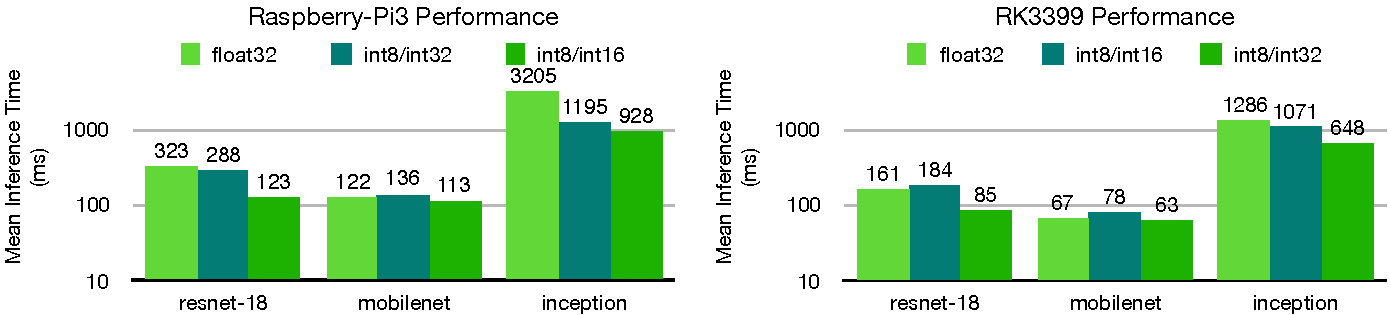
\includegraphics[width=\textwidth]{fig/eval/vision_arm.pdf}
    \caption{
      Inference time (ms) of vision DNNs on low-power platforms using
        different data types.
      Relay allows us to reduce inference time on power-constrained devices by
        easily substituting \texttt{float32} multiplications with \texttt{int8}
        multiplications and \texttt{int16} or \texttt{int32} accumulations (denoted
        at \texttt{int8}/\texttt{int16} and \texttt{int8}/\texttt{int32} respectively).
      We used 1000 trials for each model.
    }
    % \label{fig:arm-eval}
  \end{figure}

  \begin{figure}[h]
    % 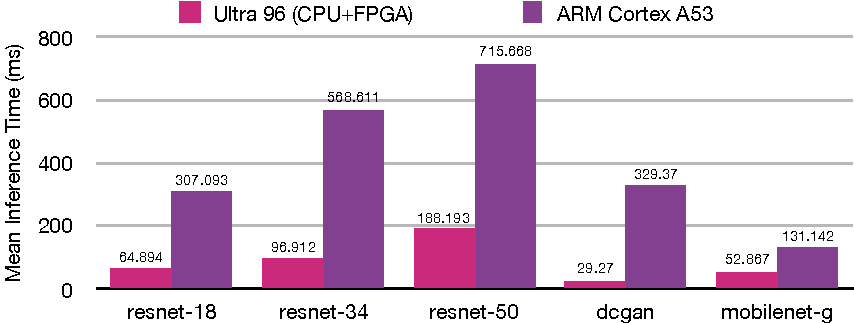
\includegraphics[width=0.6\textwidth]{fig/eval/vision_fpga.pdf}
    \caption{
      Inference time (ms) of vision DNNs on Ultra-96 FPGA-enabled SoC.
      We compare vision workloads that Relay compiles onto the embedded Cortex
        A53 CPU vs. a DNN accelerator implemented on the integrated FPGA fabric.
      Targeting DNN accelerators can unlock up to 11x speedups, but requires a
        multitude of graph-level transformations.
      We used 10 trials for each model.
    }
    % \label{fig:fpga-eval}
  \end{figure}

  Relay can handle challenging scenarios: consider edge inference where energy is a first order
    constraint due to thermal limitations or limited battery life.
  One option is to apply more aggressive quantization: instead of performing expensive
    arithmetic in the floating point domain, simpler and narrower fixed point data is used.
  Another option is hardware acceleration: instead of evaluating
    compute-intensive operations on the CPU, we can offload to a specialized accelerator.

  \paragraph{Quantized Inference on ARM CPUs and GPUs}
  We evaluate the effects of quantized inference applied by Relay on vision workloads running
  on the Raspberry-Pi3 and Firefly RK3399 ARM-based platforms.
  Figure~\ref{fig:arm-eval} shows the effects of different levels
    of quantization applied to low-power devices~\citep{roesch2019relay}.
  The numbers show that as we opt for a more aggressive quantization scheme such as \texttt{int8/16} (i.e. 8-bit multiplication and 16-bit accumulation), we achieve much improved performance.

  \paragraph{Targeting Deep Learning Accelerators on FPGAs}
  We evaluated inference time on five models including MobileNet-G \citep{mobilenet}, a grouped variant of the MobileNet architecture; ResNet-18, ResNet-34, and ResNet-50\citep{resnet}; and Deep Convolutional Generative Adversarial Networks \citep{dcgan}, a generative DNN used in unsupervised learning.
  Overall, Relay helps us efficiently offload deep learning operators onto specialized accelerators like VTA.
  Our results in Figure~\ref{fig:fpga-eval} show that we can achieve between 2.5 to 11.7$\times$ reduction in single-batch inference latency by offloading critical operators to the FPGA accelerator.
  These experiments demonstrate Relay's ability to target current and future deep learning architectures:
  \begin{enumerate}
    \item \textit{Heterogeneous FPGA/CPU offloading}: Relay lets us define the rules for offloading specific operators to the FPGA-based accelerator.
    \item \textit{Push-button quantization}: Relay can take a \texttt{fp32} model and convert its parameters to \texttt{int8} in order to enable inference on specialized accelerators.
    \item \textit{Accelerator-friendly data packing:} Relay reorganizes data so it can be effortlessly consumed by a specialized TPU-like accelerator~\citep{tpuv1}.
  \end{enumerate}

The scenario presented in the introduction demonstrates the three-pronged \textbf{extensibility challenge}
  for DL IRs:
% \begin{enumerate} % [label=\arabic*.]
%   \item \textit{Expressivity}: It should be straightforward to write models involving complex data structures (e.g., trees, graphs, and lists) and control flow.
%   \item \textit{Composability}: It should be straightforward to add and compose new optimizations
%     with existing ones (e.g., quantization, operator fusion, and automatic differentiation).
%   \item \textit{Portability}: It should be straightforward to add new hardware backends
%     (e.g., TPU, Inferentia, and FPGAs)~\citep{tpuv1, inferentia}.
% \end{enumerate}
